%
%\begin{tikzpicture}[thick,scale=0.7, every node/.style={transform shape}] \begin{axis}[
% %title={},
% %y dir=reverse, 
% %x dir=reverse, 
% ylabel={Split},
% xlabel={Alpha},
% zlabel={P@30},
% every axis/.append style={font=\large\bfseries},
% max space between ticks=25pt,
% view={-50}{20}
%% yticklabels={0k,100k}
% ] 
%
%		\addplot3[surf] coordinates { 
%%patch,patch type=biquadratic, shader=faceted,patch refines=3
%(0,1,0.4071)	(0.05,1,0.3895)	(0.1,1,0.3966)	(0.15,1,0.3975)	(0.2,1,0.3955)	(0.25,1,0.3918)	(0.3,1,0.3841)	(0.35,1,0.3751)	(0.4,1,0.3656)	(0.45,1,0.3539)	(0.5,1,0.3227)	(0.55,1,0.2764)	(0.6,1,0.2304)	(0.65,1,0.1951)	(0.7,1,0.1681)	(0.75,1,0.1434)	(0.8,1,0.1181)	(0.85,1,0.1043)	(0.9,1,0.0985)	(0.95,1,0.0905)
%
%(0,2,0.2188)	(0.05,2,0.2241)	(0.1,2,0.2322)	(0.15,2,0.2324)	(0.2,2,0.2317)	(0.25,2,0.2281)	(0.3,2,0.2275)	(0.35,2,0.2253)	(0.4,2,0.2191)	(0.45,2,0.2102)	(0.5,2,0.197)	(0.55,2,0.1859)	(0.6,2,0.1599)	(0.65,2,0.1417)	(0.7,2,0.1324)	(0.75,2,0.113)	(0.8,2,0.1025)	(0.85,2,0.0908)	(0.9,2,0.0876)	(0.95,2,0.0832)
%
%(0,3,0.1814)	(0.05,3,0.1878)	(0.1,3,0.1978)	(0.15,3,0.2)	(0.2,3,0.2014)	(0.25,3,0.2026)	(0.3,3,0.2027)	(0.35,3,0.2023)	(0.4,3,0.1993)	(0.45,3,0.193)	(0.5,3,0.1859)	(0.55,3,0.1707)	(0.6,3,0.1521)	(0.65,3,0.1322)	(0.7,3,0.1187)	(0.75,3,0.1006)	(0.8,3,0.0853)	(0.85,3,0.0748)	(0.9,3,0.0716)	(0.95,3,0.0685)
%
%(0,4,0.3427)	(0.05,4,0.3334)	(0.1,4,0.3351)	(0.15,4,0.3361)	(0.2,4,0.3366)	(0.25,4,0.3366)	(0.3,4,0.3364)	(0.35,4,0.3339)	(0.4,4,0.3273)	(0.45,4,0.315)	(0.5,4,0.2927)	(0.55,4,0.2695)	(0.6,4,0.2312)	(0.65,4,0.1978)	(0.7,4,0.1686)	(0.75,4,0.1426)	(0.8,4,0.1141)	(0.85,4,0.0998)	(0.9,4,0.0929)	(0.95,4,0.0874)
%
%(0,5,0.3696)	(0.05,5,0.382)	(0.1,5,0.3856)	(0.15,5,0.3867)	(0.2,5,0.3857)	(0.25,5,0.3833)	(0.3,5,0.379)	(0.35,5,0.3763)	(0.4,5,0.367)	(0.45,5,0.3549)	(0.5,5,0.3346)	(0.55,5,0.3068)	(0.6,5,0.2717)	(0.65,5,0.2308)	(0.7,5,0.2057)	(0.75,5,0.1727)	(0.8,5,0.1506)	(0.85,5,0.1338)	(0.9,5,0.1251)	(0.95,5,0.1178)
%
%
%}; \end{axis} \end{tikzpicture}

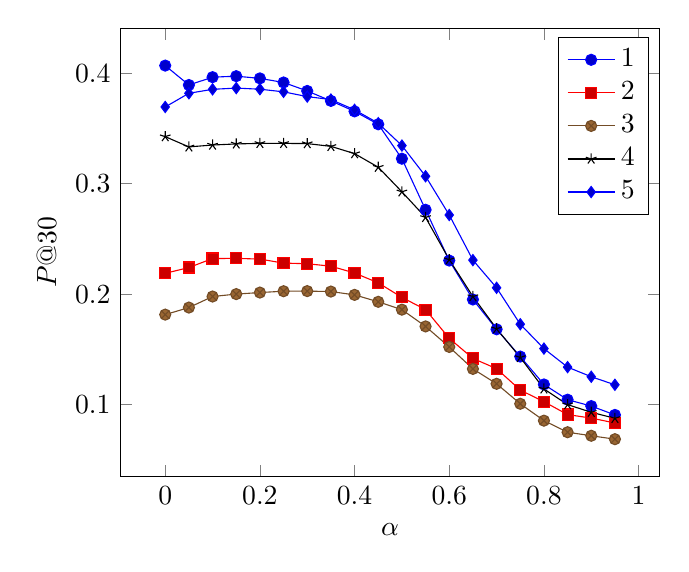
\begin{tikzpicture}
\begin{axis}[
	xlabel={$\alpha$},
	ylabel={$P@30$}
]
\addplot coordinates {
	(0,0.4071)	(0.05,0.3895)	(0.1,0.3966)	(0.15,0.3975)	(0.2,0.3955)	(0.25,0.3918)	(0.3,0.3841)	(0.35,0.3751)	(0.4,0.3656)	(0.45,0.3539)	(0.5,0.3227)	(0.55,0.2764)	(0.6,0.2304)	(0.65,0.1951)	(0.7,0.1681)	(0.75,0.1434)	(0.8,0.1181)	(0.85,0.1043)	(0.9,0.0985)	(0.95,0.0905)
};

\addplot coordinates{	
	(0,0.2188)	(0.05,0.2241)	(0.1,0.2322)	(0.15,0.2324)	(0.2,0.2317)	(0.25,0.2281)	(0.3,0.2275)	(0.35,0.2253)	(0.4,0.2191)	(0.45,0.2102)	(0.5,0.197)	(0.55,0.1859)	(0.6,0.1599)	(0.65,0.1417)	(0.7,0.1324)	(0.75,0.113)	(0.8,0.1025)	(0.85,0.0908)	(0.9,0.0876)	(0.95,0.0832)
};

\addplot coordinates{
	(0,0.1814)	(0.05,0.1878)	(0.1,0.1978)	(0.15,0.2)	(0.2,0.2014)	(0.25,0.2026)	(0.3,0.2027)	(0.35,0.2023)	(0.4,0.1993)	(0.45,0.193)	(0.5,0.1859)	(0.55,0.1707)	(0.6,0.1521)	(0.65,0.1322)	(0.7,0.1187)	(0.75,0.1006)	(0.8,0.0853)	(0.85,0.0748)	(0.9,0.0716)	(0.95,0.0685)
};

\addplot coordinates{
	(0,0.3427)	(0.05,0.3334)	(0.1,0.3351)	(0.15,0.3361)	(0.2,0.3366)	(0.25,0.3366)	(0.3,0.3364)	(0.35,0.3339)	(0.4,0.3273)	(0.45,0.315)	(0.5,0.2927)	(0.55,0.2695)	(0.6,0.2312)	(0.65,0.1978)	(0.7,0.1686)	(0.75,0.1426)	(0.8,0.1141)	(0.85,0.0998)	(0.9,0.0929)	(0.95,0.0874)
};

\addplot coordinates{
		(0,0.3696)	(0.05,0.382)	(0.1,0.3856)	(0.15,0.3867)	(0.2,0.3857)	(0.25,0.3833)	(0.3,0.379)	(0.35,0.3763)	(0.4,0.367)	(0.45,0.3549)	(0.5,0.3346)	(0.55,0.3068)	(0.6,0.2717)	(0.65,0.2308)	(0.7,0.2057)	(0.75,0.1727)	(0.8,0.1506)	(0.85,0.1338)	(0.9,0.1251)	(0.95,0.1178)
};
\legend{$1$,$2$,$3$,$4$,$5$}
\end{axis}
\end{tikzpicture}